\documentclass[level=3]{kidscode}
%% A paper CRC card (Class / Responsibilities / Collaborators)
\newcommand{\crccard}{\par\noindent
  %% alt: An empty class card with a space for the class name, a left column for responsibilities (what it knows and does) and a right column for collaborators (who it works with).
  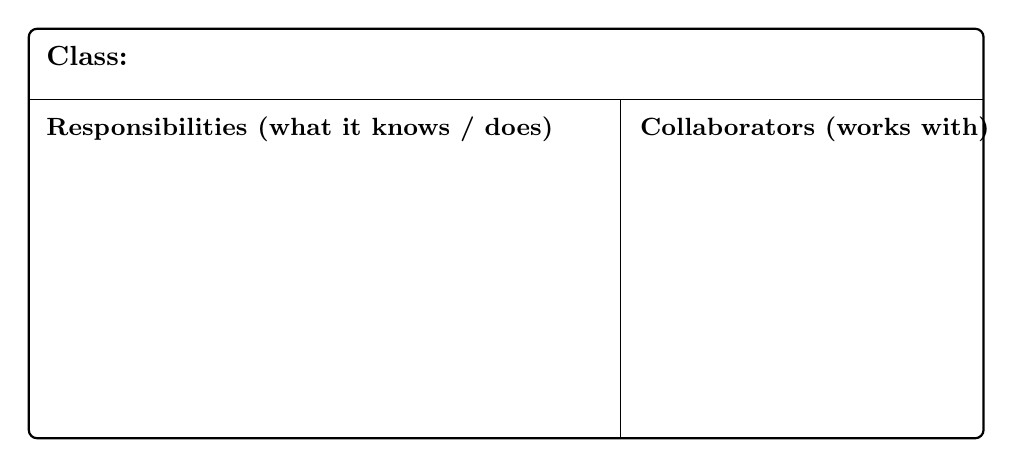
\begin{tikzpicture}
    \draw[thick, rounded corners=3pt] (0,0) rectangle (\linewidth,-5.2);
    \draw (0,-0.9) -- (\linewidth,-0.9);
    \draw (0.62\linewidth,-0.9) -- (0.62\linewidth,-5.2);
    \node[anchor=north west, font=\bfseries] at (0.1,-0.1) {Class:};
    \node[anchor=north west, font=\small\bfseries] at (0.1,-1.0) {Responsibilities (what it knows / does)};
    \node[anchor=north west, font=\small\bfseries] at (0.63\linewidth,-1.0) {Collaborators (works with)};
  \end{tikzpicture}\par\medskip}

\begin{document}
\kctitle{Project Brief: Build Something Big}{Your Level 3 final project, from idea to showcase}
\namedateline

\begin{tip}[What is this?]
From week 9 to week 12 you will design and build a program that is bigger than anything you have
made so far --- and you will build it like real software makers do: plan first, save your
progress with git, test it with pytest, ask people to try it, and explain your design. You can
work alone or in a pair.
\end{tip}

\section{1. Choose your option}

\renewcommand{\arraystretch}{1.3}
\begin{tabularx}{\linewidth}{@{}>{\bfseries\raggedright\arraybackslash}p{3.1cm}X>{\raggedright\arraybackslash}p{3.6cm}@{}}
\toprule
\rowcolor{kcaccent!15} Option & What you make & Start from\\ \midrule
(a) Grid game & A game on a grid of squares: a maze, a dungeon, a puzzle, a farm. Characters are
objects; enemies can use an algorithm to move. & \texttt{grid\_game\_template.py}\\ \midrule
(b) Generative art app & An app that makes pictures from rules: fractals, patterns, tiles. Shapes
are objects; your art can be saved and loaded again. & \texttt{art\_app\_template.py}\\ \midrule
(c) Data / AI app & An app that answers questions about data, draws charts, or predicts things
with a nearest-neighbor \enquote{AI}. & \texttt{data\_app\_template.py} and \texttt{data/games.csv}\\
\bottomrule
\end{tabularx}

The templates are in the \texttt{starter} folder. They already run; the \texttt{README.md} there
tells you how to copy the folder and make your first git commit.

\section{2. The must-haves}

Whatever you build, your finished project must have all of these. Check them off as you go.

\begin{selfcheck}
  \item \textbf{At least 2 classes} that you wrote, and one of them uses \textbf{inheritance}
        (\py|class Dragon(Character):|) or \textbf{composition} (a class that has other objects).
  \item A \textbf{data structure beyond a flat list}: a dictionary, a stack or queue, or a 2D grid.
  \item One \textbf{named algorithm}: a search, a sort, recursion, or breadth-first search (BFS).
  \item A \textbf{saved file}: high scores, a level, saved art or results, created if it is missing.
  \item At least \textbf{5 pytest tests} that pass.
  \item A \textbf{git history with 8 or more meaningful commits} (small steps with clear messages).
  \item A short \textbf{README.md}: what it is, how to run it, how it is built, credits.
  \item \textbf{Fair and safe}: nicknames only, no personal data, never color alone (use shapes,
        letters or words too), credit for anything you did not make.
\end{selfcheck}

\section{3. Idea menu}
Pick one, mix two, or invent your own. Small and finished beats huge and broken!

\begin{longtable}{@{}>{\raggedright\arraybackslash}p{\dimexpr(\linewidth-4\tabcolsep)/3}>{\raggedright\arraybackslash}p{\dimexpr(\linewidth-4\tabcolsep)/3}>{\raggedright\arraybackslash}p{\dimexpr(\linewidth-4\tabcolsep)/3}@{}}
\toprule
\rowcolor{kcaccent!15}\textbf{(a) Grid games} & \textbf{(b) Generative art} & \textbf{(c) Data / AI}\\ \midrule\endhead
\bottomrule\endfoot
Dungeon crawler: collect keys, open doors, a monster that hunts you with BFS &
Fractal forest: trees with different depth, angle and season palettes; save your favorite settings &
Game-night stats: survey your family's favorite games, clean the data, chart it\\ \midrule
Sokoban-style box pusher with levels in text files and an undo stack &
Quilt maker: tiles of shape classes in a grid, mirror and rotate rules &
Monster sorter: a nearest-neighbor AI guesses the type of a new monster from its features\\ \midrule
Snake on a grid with a queue for the body &
Flood-fill coloring book: click a region to fill it (recursion or BFS) &
Weather or reading log: average, best week, a bar chart, a prediction\\ \midrule
Farm or garden simulator: plants are objects that grow each tick &
Spirograph studio: pattern classes, sliders by keys, a gallery saved as JSON &
Story maker: a Markov text generator trained on your own stories\\
\end{longtable}

\section{4. Milestones}

\begin{longtable}{@{}>{\bfseries\raggedright\arraybackslash}p{3.0cm}>{\raggedright\arraybackslash}p{2.6cm}p{\dimexpr\linewidth-5.6cm-4\tabcolsep}@{}}
\toprule
\rowcolor{kcaccent!15} Milestone & When & Done when\ldots\\ \midrule\endhead
\bottomrule\endfoot
M1 Pitch & end of week 9 & Your pitch page (section 5) is filled in and your teacher has said
\enquote{go}.\\ \midrule
M2 Design + core classes & week 10 & CRC cards and a class diagram are drawn. Your project folder is a git
repository. Your main classes exist in code and run without errors. At least 2 commits in the
session and 3 more at home; a first test is a bonus.\\ \midrule
M3 Features + 5 tests + playtest & week 11, first half & The must-have features work, 5+ tests
pass, and someone else has playtested it (feedback card filled in).\\ \midrule
M4 README + polish & week 11, second half & You fixed the top bugs from the playtest, wrote the
README, and have 6+ meaningful commits (8+ by the showcase).\\ \midrule
Showcase & week 12 & You show your project and explain one design decision.\\
\end{longtable}

\begin{tip}[Commit like a pro]
Commit every time something small works: \texttt{"Add Hero class"}, \texttt{"Stop hero walking
through walls"}, \texttt{"Test that treasure adds 1 point"}. Messages like \texttt{"stuff"} or
\texttt{"final"} do not count as meaningful.
\end{tip}

\section{5. Design pages}

\subsection{Page A: My pitch (M1)}
\renewcommand{\arraystretch}{2.1}
\begin{tabularx}{\linewidth}{@{}>{\bfseries}p{5.2cm}X@{}}
Project name & \hrulefill\\
Option (a, b or c) & \hrulefill\\
In one sentence, it is\ldots & \hrulefill\\
It is for (who will enjoy it?) & \hrulefill\\
Must-have feature 1 & \hrulefill\\
Must-have feature 2 & \hrulefill\\
Must-have feature 3 & \hrulefill\\
Nice-to-have (if there is time) & \hrulefill\\
My algorithm (and what it does) & \hrulefill\\
My data structure (and what it holds) & \hrulefill\\
The file it saves & \hrulefill\\
\end{tabularx}

\clearpage
\subsection{Page B: CRC cards (M2)}
Write one card for each class. \textbf{Responsibilities} are what it knows (attributes) and does
(methods). \textbf{Collaborators} are the other classes it uses.

\begin{workedexample}[A CRC card for a grid game]
\textbf{Class:} Dragon \quad \textbf{Responsibilities:} knows its position and speed; chooses the
next square using BFS; can say if it caught the hero. \quad \textbf{Collaborators:} Grid (to find
open squares), Hero (where to go). \textbf{Is a} Character (inherits position and
\texttt{move}).
\end{workedexample}
\crccard
\crccard
\crccard

\clearpage
\subsection{Page C: Class diagram}
Draw a box for each class (name, attributes, methods). Draw an arrow with an \textbf{open
triangle} for \enquote{is a} (inheritance) and a line with a \textbf{diamond} for \enquote{has a}
(composition). Example:

\begin{center}
%% alt: A class diagram. Hero and Dragon each point up to Character with an is-a arrow. Character has pos and move(direction). A Game has characters (grid, hero, dragons and tick()) and also has a Grid with cells and neighbors(). Hero adds treasure and collect(). Dragon adds speed and choose_step().
\begin{tikzpicture}[
  cls/.style={draw, thick, rounded corners=2pt, align=left, font=\small, fill=kcsky!10, inner sep=4pt},
  isa/.style={-{Triangle[open,length=7pt,width=7pt]}, thick},
  hasa/.style={{Diamond[length=9pt,width=6pt]}-, thick}]
  \node[cls] (char) at (0,0) {\textbf{Character}\\ pos\\ move(direction)};
  \node[cls] (hero) at (-2.6,-2.5) {\textbf{Hero}\\ treasure\\ collect()};
  \node[cls] (dragon) at (2.6,-2.5) {\textbf{Dragon}\\ speed\\ choose\_step()};
  \node[cls] (game) at (7.2,0) {\textbf{Game}\\ grid, hero, dragons\\ tick()};
  \node[cls] (grid) at (7.2,-2.5) {\textbf{Grid}\\ cells\\ neighbors()};
  \draw[isa] (hero.north) -- node[left, font=\scriptsize] {is a} (char.south west);
  \draw[isa] (dragon.north) -- node[right, font=\scriptsize] {is a} (char.south east);
  \draw[hasa] (game.west) -- node[above, font=\scriptsize] {has} (char.east);
  \draw[hasa] (game.south) -- node[right, font=\scriptsize] {has a} (grid.north);
\end{tikzpicture}
\end{center}
\answerspace{7cm}

\subsection{Page D: My milestone plan}
\renewcommand{\arraystretch}{1.9}
\begin{tabularx}{\linewidth}{@{}|>{\bfseries}p{2.6cm}|p{2.2cm}|X|@{}}
\hline
\rowcolor{kcaccent!15} Milestone & Date & What will work (and which commits I expect)\\ \hline
M1 Pitch & & \\ \hline
M2 Design & & \\ \hline
M3 Features & & \\ \hline
M4 Polish & & \\ \hline
Showcase & & \\ \hline
\end{tabularx}

\section{6. Testing your project}
Test the \textbf{logic}, not the drawing. Keep rules (moving, scoring, saving, sorting, predicting)
in classes and functions that do not use turtle, and keep the turtle code in its own part. Ideas:
\begin{itemize}[itemsep=1pt]
  \item a wall blocks a move; collecting treasure adds a point;
  \item your search or sort gives the right answer on a tiny example \emph{and} an edge case
        (empty list, unreachable square);
  \item saving and loading gives back the same data (use pytest's \py|tmp_path| folder);
  \item your classifier predicts the right label for an obvious example.
\end{itemize}
\texttt{test\_my\_project.py} in the starter folder has examples. Run your tests from Thonny's
\menu{Tools} $\rightarrow$ \menu{Open system shell\ldots} with \texttt{python -m pytest -q}.

\section{7. Playtest feedback card}
Give this to your playtester (week 11). Then fix the most important thing first.

\begin{reflection}[Playtest card]
Project: \rule{5cm}{0.4pt} \quad Playtester (nickname): \rule{4cm}{0.4pt}\par
\textbf{Star 1} (something great): \answerlines{1}
\textbf{Star 2} (something else great): \answerlines{1}
\textbf{A wish} (one thing to improve): \answerlines{1}
Did anything confuse you or break? Could someone who is color-blind play it? \answerlines{1}
\end{reflection}

\section{8. How your project is judged}
Your teacher uses the same rubric. Before the showcase, check one box in each row: where do \emph{you} think you are?

\begingroup\small
\renewcommand{\arraystretch}{1.3}
\begin{longtable}{@{}>{\bfseries\raggedright\arraybackslash}p{2.2cm}>{\raggedright\arraybackslash}p{3.15cm}>{\raggedright\arraybackslash}p{3.15cm}>{\raggedright\arraybackslash}p{3.15cm}>{\raggedright\arraybackslash}p{\dimexpr\linewidth-11.65cm-8\tabcolsep}@{}}
\toprule
\rowcolor{kcaccent!15} & Just starting & Getting there & Got it & Expert\\ \midrule\endhead
\bottomrule\endfoot
Creativity & $\square$ My idea is a copy of an example & $\square$ I changed an example a bit & $\square$ My project has my own idea and style & $\square$ My project surprises people with something new\\ \midrule
Working code & $\square$ It crashes often & $\square$ It runs, with some bugs & $\square$ All must-have features work & $\square$ It works well, even when people do unexpected things\\ \midrule
Design / OOP & $\square$ One class, or classes that do not help & $\square$ 2 classes, but jobs are mixed up & $\square$ Clear classes; inheritance or composition used well & $\square$ I can show why my class design makes the code easier to change\\ \midrule
Testing & $\square$ Fewer than 3 tests & $\square$ 3--4 tests, or tests that fail & $\square$ 5+ passing tests of my logic & $\square$ My tests include edge cases and caught a real bug\\ \midrule
Git history & $\square$ Fewer than 4 commits & $\square$ 4--7 commits, or unclear messages & $\square$ 8+ commits with clear messages & $\square$ My log tells the story of my project step by step\\ \midrule
Explaining design decisions & $\square$ I can show what it does & $\square$ I can explain how one part works & $\square$ I can explain why I chose my design & $\square$ I can compare my design with another way and explain the trade-off\\
\end{longtable}
\endgroup

\section{9. Need more time, or want more?}
\begin{differentiation}
\supportpath Start from a starter template and keep it small: 2 classes, 3 features, 5 simple tests
(one per method). Ask your teacher for a \enquote{feature card} with one small step at a time. It
is fine to finish fewer features well.
\extensionpath Add a second level or mode loaded from a file; write tests \emph{before} the code
(test-first); use BFS or recursion in a second place; add a settings dictionary saved as JSON; try
k-nearest neighbors (3 vote) for option (c).
\end{differentiation}

\section{10. Showcase: your 2-minute talk}
Use the talk card in workbook chapter 12. Pick \textbf{one} design decision.
\begin{checklist}
  \item \textbf{What} is it and who is it for? Show the best feature. (40 seconds)
  \item \textbf{Problem}: what was hard or not working? (20 seconds)
  \item \textbf{Choice} and \textbf{Why}: what you chose, another way you could have done it,
        and why you chose yours (a bug a test caught is a great story too). (45 seconds)
  \item \textbf{Next time}: what you would change or add. (15 seconds)
\end{checklist}

\begin{safety}[Showcase safety]
Show your nickname, never your real name, on screen. Photos or videos only if everyone agrees.
Your project stays on our computers; we do not upload it anywhere.
\end{safety}
\end{document}
